\documentclass[10pt]{article}
% Built from REPORT.md (the source of truth) with the homework template's preamble.
\usepackage[T1]{fontenc}
\usepackage[utf8]{inputenc}
\usepackage{lmodern}
\usepackage{amsmath,amsfonts,amsthm,amssymb}
\usepackage{fancyhdr}
\usepackage{lastpage}
\usepackage{extramarks}
\usepackage{chngpage}
\usepackage{soul,color}
\usepackage{graphicx,float,wrapfig}
\usepackage{booktabs}
\usepackage{caption}
\usepackage{enumitem}
\usepackage{titlesec}
\usepackage{microtype}
\usepackage[hidelinks]{hyperref}

% Margins as in the template
\topmargin=-0.45in      %
\evensidemargin=0in     %
\oddsidemargin=0in      %
\textwidth=6.5in        %
\textheight=9.0in       %
\headsep=0.25in         %
\headheight=13pt        %

% Homework Specific Information
\newcommand{\hmwkTitle}{Tally: AI Screening for Finance \&\ Accounting}
\newcommand{\hmwkDueDate}{17\ Oct\ 2026}
\newcommand{\hmwkClass}{HYT Graduate 2027 Take-Home}
% >>> FILL IN YOUR NAME ON THE NEXT LINE <<<
\newcommand{\hmwkAuthorName}{Vaibhavi Dhokale}

% Setup the header and footer
\pagestyle{fancy}                                                       %
\lhead{\hmwkAuthorName}                                                 %
\chead{}
\rhead{\hmwkClass: \hmwkTitle}
\lfoot{\lastxmark}                                                      %
\cfoot{}
\rfoot{Page\ \thepage\ of\ \pageref{LastPage}}                          %
\renewcommand\headrulewidth{0.4pt}                                      %
\renewcommand\footrulewidth{0.4pt}                                      %

%%%%%%%%%%%%%%%%%%%%%%%%%%%%%%%%%%%%%%%%%%%%%%%%%%%%%%%%%%%%%
% Some tools (from the template)
\newcommand{\enterProblemHeader}[1]{\nobreak\extramarks{#1}{#1 continued on next page\ldots}\nobreak%
                                    \nobreak\extramarks{#1 (continued)}{#1 continued on next page\ldots}\nobreak}%
\newcommand{\exitProblemHeader}[1]{\nobreak\extramarks{#1 (continued)}{#1 continued on next page\ldots}\nobreak%
                                   \nobreak\extramarks{#1}{}\nobreak}%

\setcounter{secnumdepth}{0}
\newcommand{\homeworkProblemName}{}%
\newcounter{homeworkProblemCounter}%
\newenvironment{homeworkProblem}[1][Problem \arabic{homeworkProblemCounter}]%
  {\stepcounter{homeworkProblemCounter}%
   \renewcommand{\homeworkProblemName}{#1}%
   \section{\homeworkProblemName}%
   \enterProblemHeader{\homeworkProblemName}}%
  {\exitProblemHeader{\homeworkProblemName}}%
%%%%%%%%%%%%%%%%%%%%%%%%%%%%%%%%%%%%%%%%%%%%%%%%%%%%%%%%%%%%%

% Compact spacing (fonts and margins unchanged)
\titlespacing*{\section}{0pt}{6pt plus 2pt minus 1pt}{2pt}
\titleformat*{\section}{\large\bfseries}
\setlist{nosep,leftmargin=1.2em}
\setlength{\parskip}{2pt}
\setlength{\parindent}{0pt}
\setlength{\abovecaptionskip}{2pt}
\setlength{\textfloatsep}{6pt plus 2pt}
\setlength{\intextsep}{4pt plus 2pt}
\newcommand{\tablefont}{\small}
\newcommand{\code}[1]{\texttt{#1}}
\newcommand{\best}[1]{\textbf{#1}}

\begin{document}

% Compact title block (replaces the template's title page and contents)
\begin{center}
  {\Large\textbf{\hmwkTitle}}\\[2pt]
  \hmwkClass\ \textbar\ Due \hmwkDueDate\ \textbar\ \textbf{\hmwkAuthorName}
\end{center}
\vspace{-4pt}

Job family: \textbf{finance \& accounting}. Data: 12 real LinkedIn postings (Kaggle \emph{arshkon}) and 295 real resumes (Kaggle \emph{snehaanbhawal}). Golden set: 180 labelled (job, resume) pairs, with \textbf{3 dev jobs (45 pairs)} used for every tuning choice and \textbf{9 test jobs (135 pairs)} used only for reporting. Every number comes from \code{results/*.json} and is regenerated by \code{make reproduce}.

\smallskip
\noindent\fbox{\begin{minipage}{\dimexpr\linewidth-2\fboxsep-2\fboxrule}
\textbf{Label status.} The 180 relevance/decision labels are \textbf{human}: written blind from the text packets, without system output (\code{golden/labels.csv}). The 30 explanation ratings the judge is compared with are \textbf{human} too (\code{golden/explanation\_ratings.csv}). Claude Sonnet drafts of both are kept as second raters (\S3, \S7). Still AI-drafted: the JD/extraction gold (\S6). Headline numbers use Claude Sonnet as the pipeline's LLM; \S11 re-runs everything on two Gemini models, including the production setting, \code{gemini-3.5-flash-lite}.
\end{minipage}}

%----------------------------------------------------------------------------
\begin{homeworkProblem}[1. Problem framing]
A recruiter with 15--300 applicants wants a \textbf{short list they can trust}, and the guarantee that \textbf{nobody good is quietly dropped}. So Tally only ever \emph{promotes} (Shortlist) or \emph{routes to a human} (Needs review / Low priority), and every line of its reasoning is a checklist item with a quote. Missing a good candidate is costed at 5$\times$ shortlisting a weak one.

\textbf{Not built}: auto-reject; an LLM that outputs a score; OCR for scanned PDFs (text-layer PDFs and pasted job descriptions are supported); multi-family support; learning-to-rank (180 labels is not enough to train on and still evaluate honestly).
\end{homeworkProblem}

%----------------------------------------------------------------------------
\begin{homeworkProblem}[2. System]
Posting $\rightarrow$ LLM checklist (4--10 requirements: must/nice, category, years/degree, source quote). Resume $\rightarrow$ clean (NFKC, invisible characters, PII mask, injection regex) $\rightarrow$ LLM profile (roles with dates, degrees, certifications). Per requirement, years and degree are compared \textbf{in code}; everything else is graded by the LLM \textbf{from the 5 resume passages BM25 retrieves for it}, with a verbatim quote that code verifies (no match $\rightarrow$ zero credit + review). Score $= \Sigma\,\text{weight}\cdot\text{credit} / \Sigma\,\text{weight}$ (must $\times2$, nice $\times1$; met 1, partial $\tfrac12$, not met 0).

\textbf{Lanes.} \emph{Shortlist}: score $\geq 0.525$, at most one must-have not fully met, no blocking flag. \emph{Low priority}: score $< 0.35$ with a must-have missing and no blocking flag. \emph{Needs review}: everything else, with reason codes (\code{MUST\_NOT\_MET}, \code{MUST\_PARTIAL}, \code{BORDERLINE}, \code{INJECTION}, \code{KEYWORD\_STUFFING}, \code{UNVERIFIED\_QUOTE}, \code{DATES\_UNCLEAR}, \code{THIN\_RESUME}; \code{LOCATION} is information only). The one allowed gap is always named in the explanation as ``Ask about: \ldots''.

\begin{figure}[H]\centering
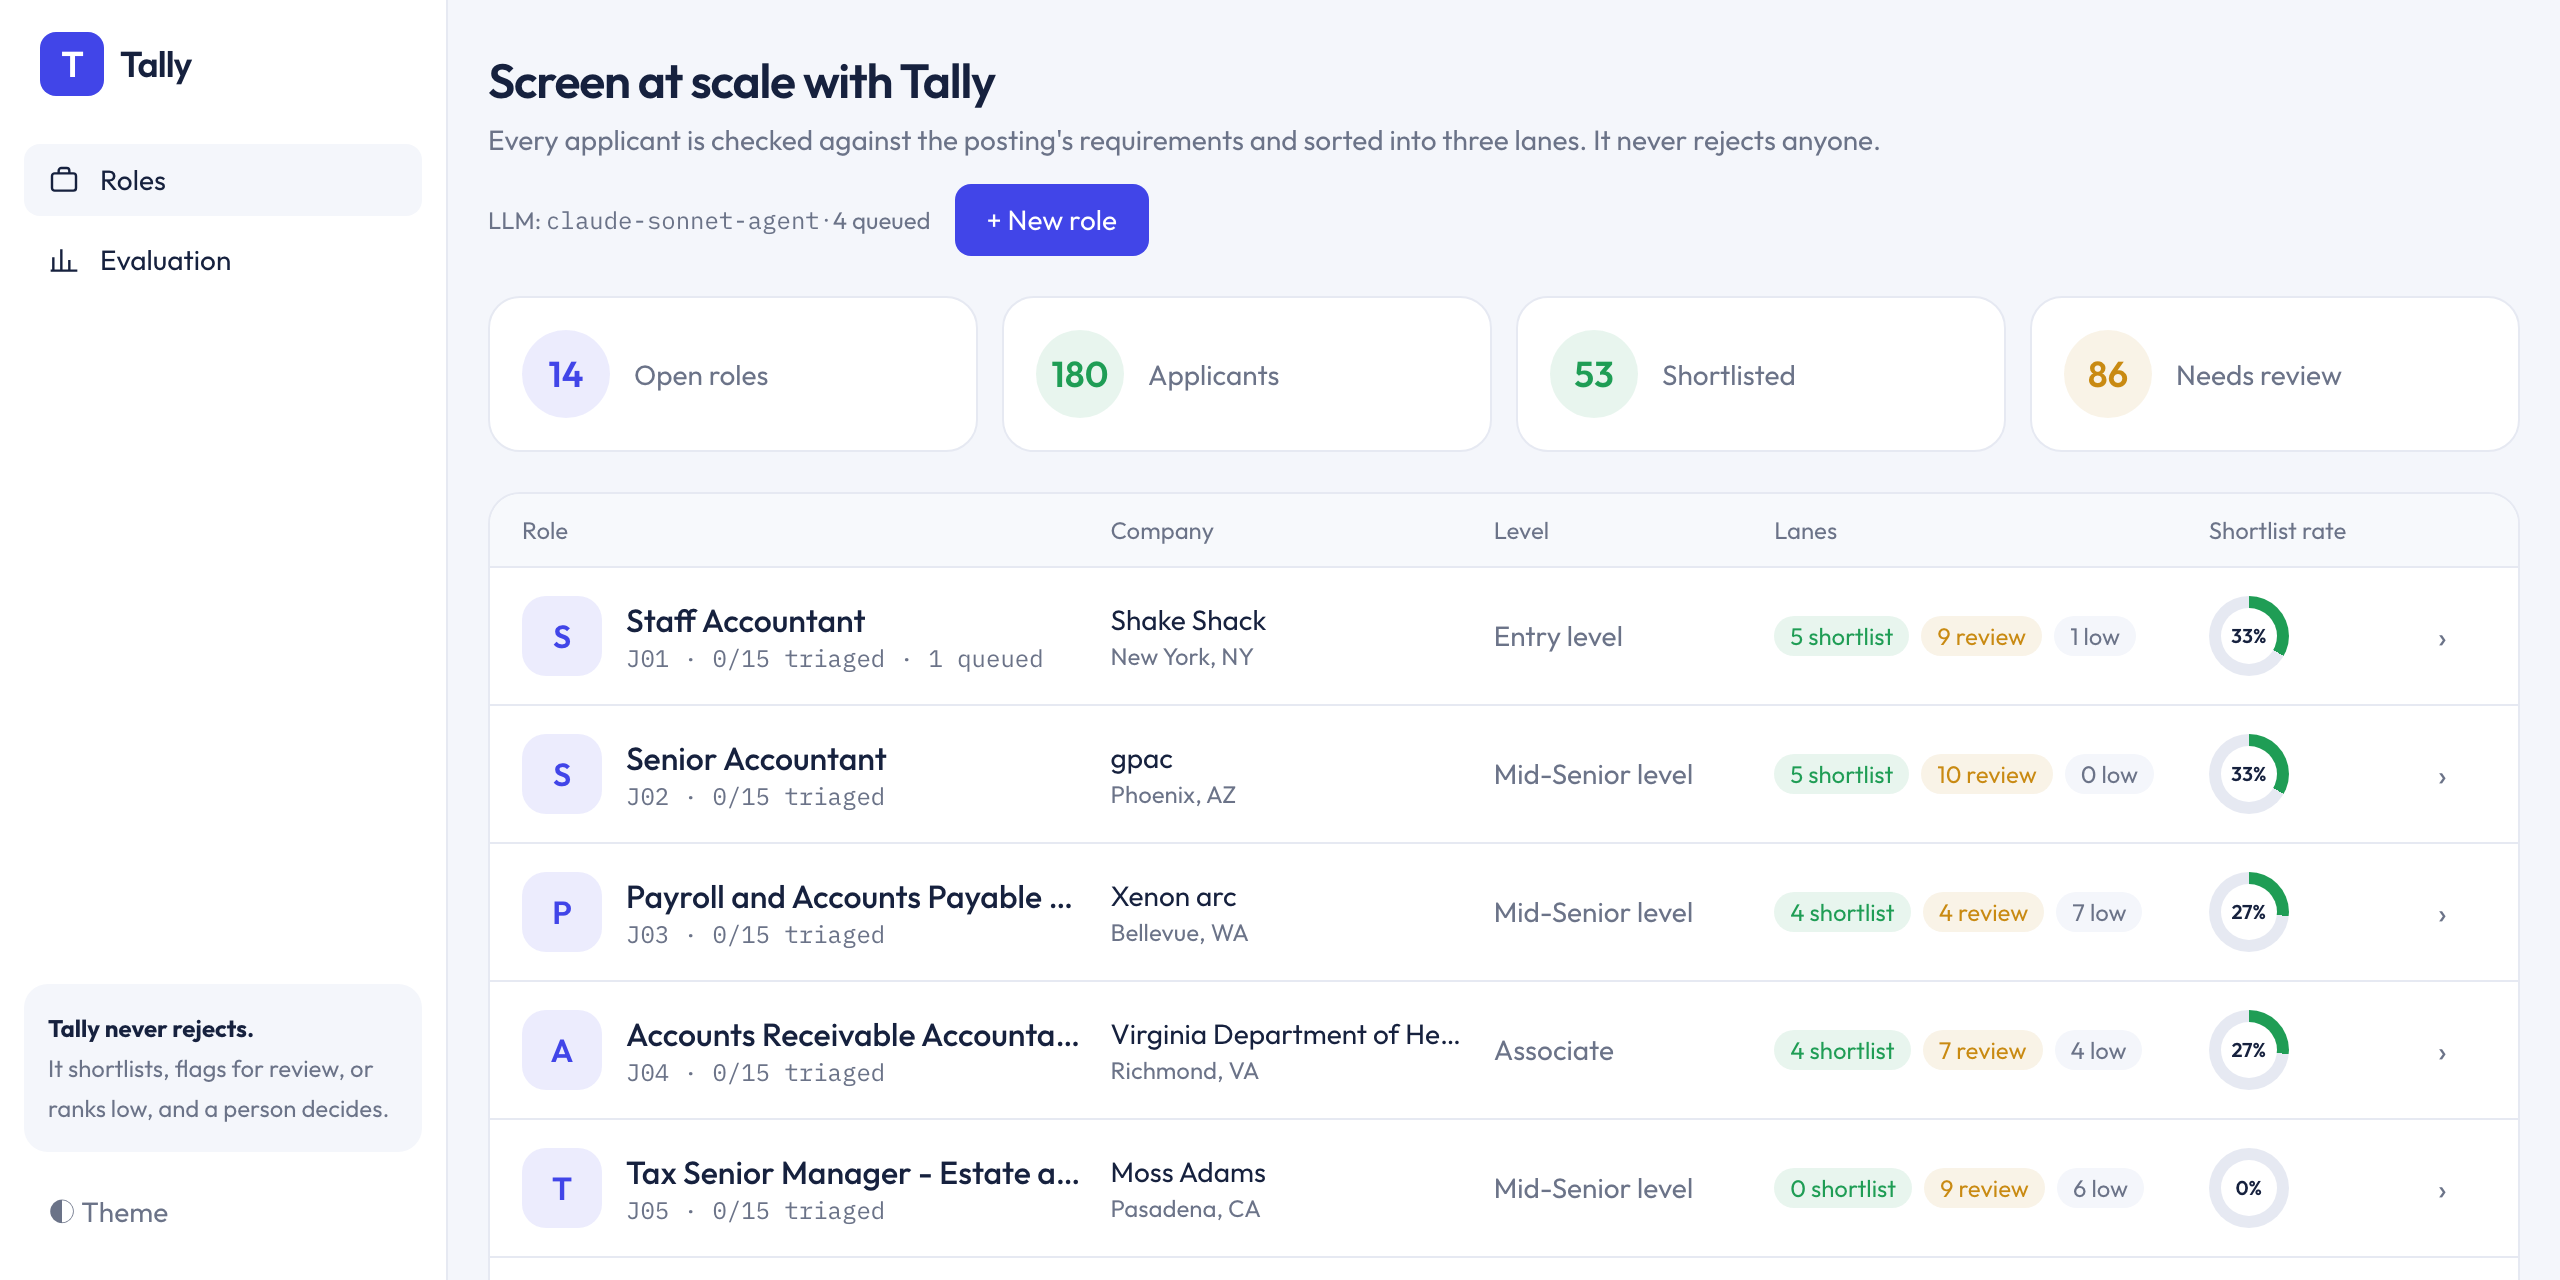
\includegraphics[width=0.49\linewidth]{docs/ui_dash.png}\hfill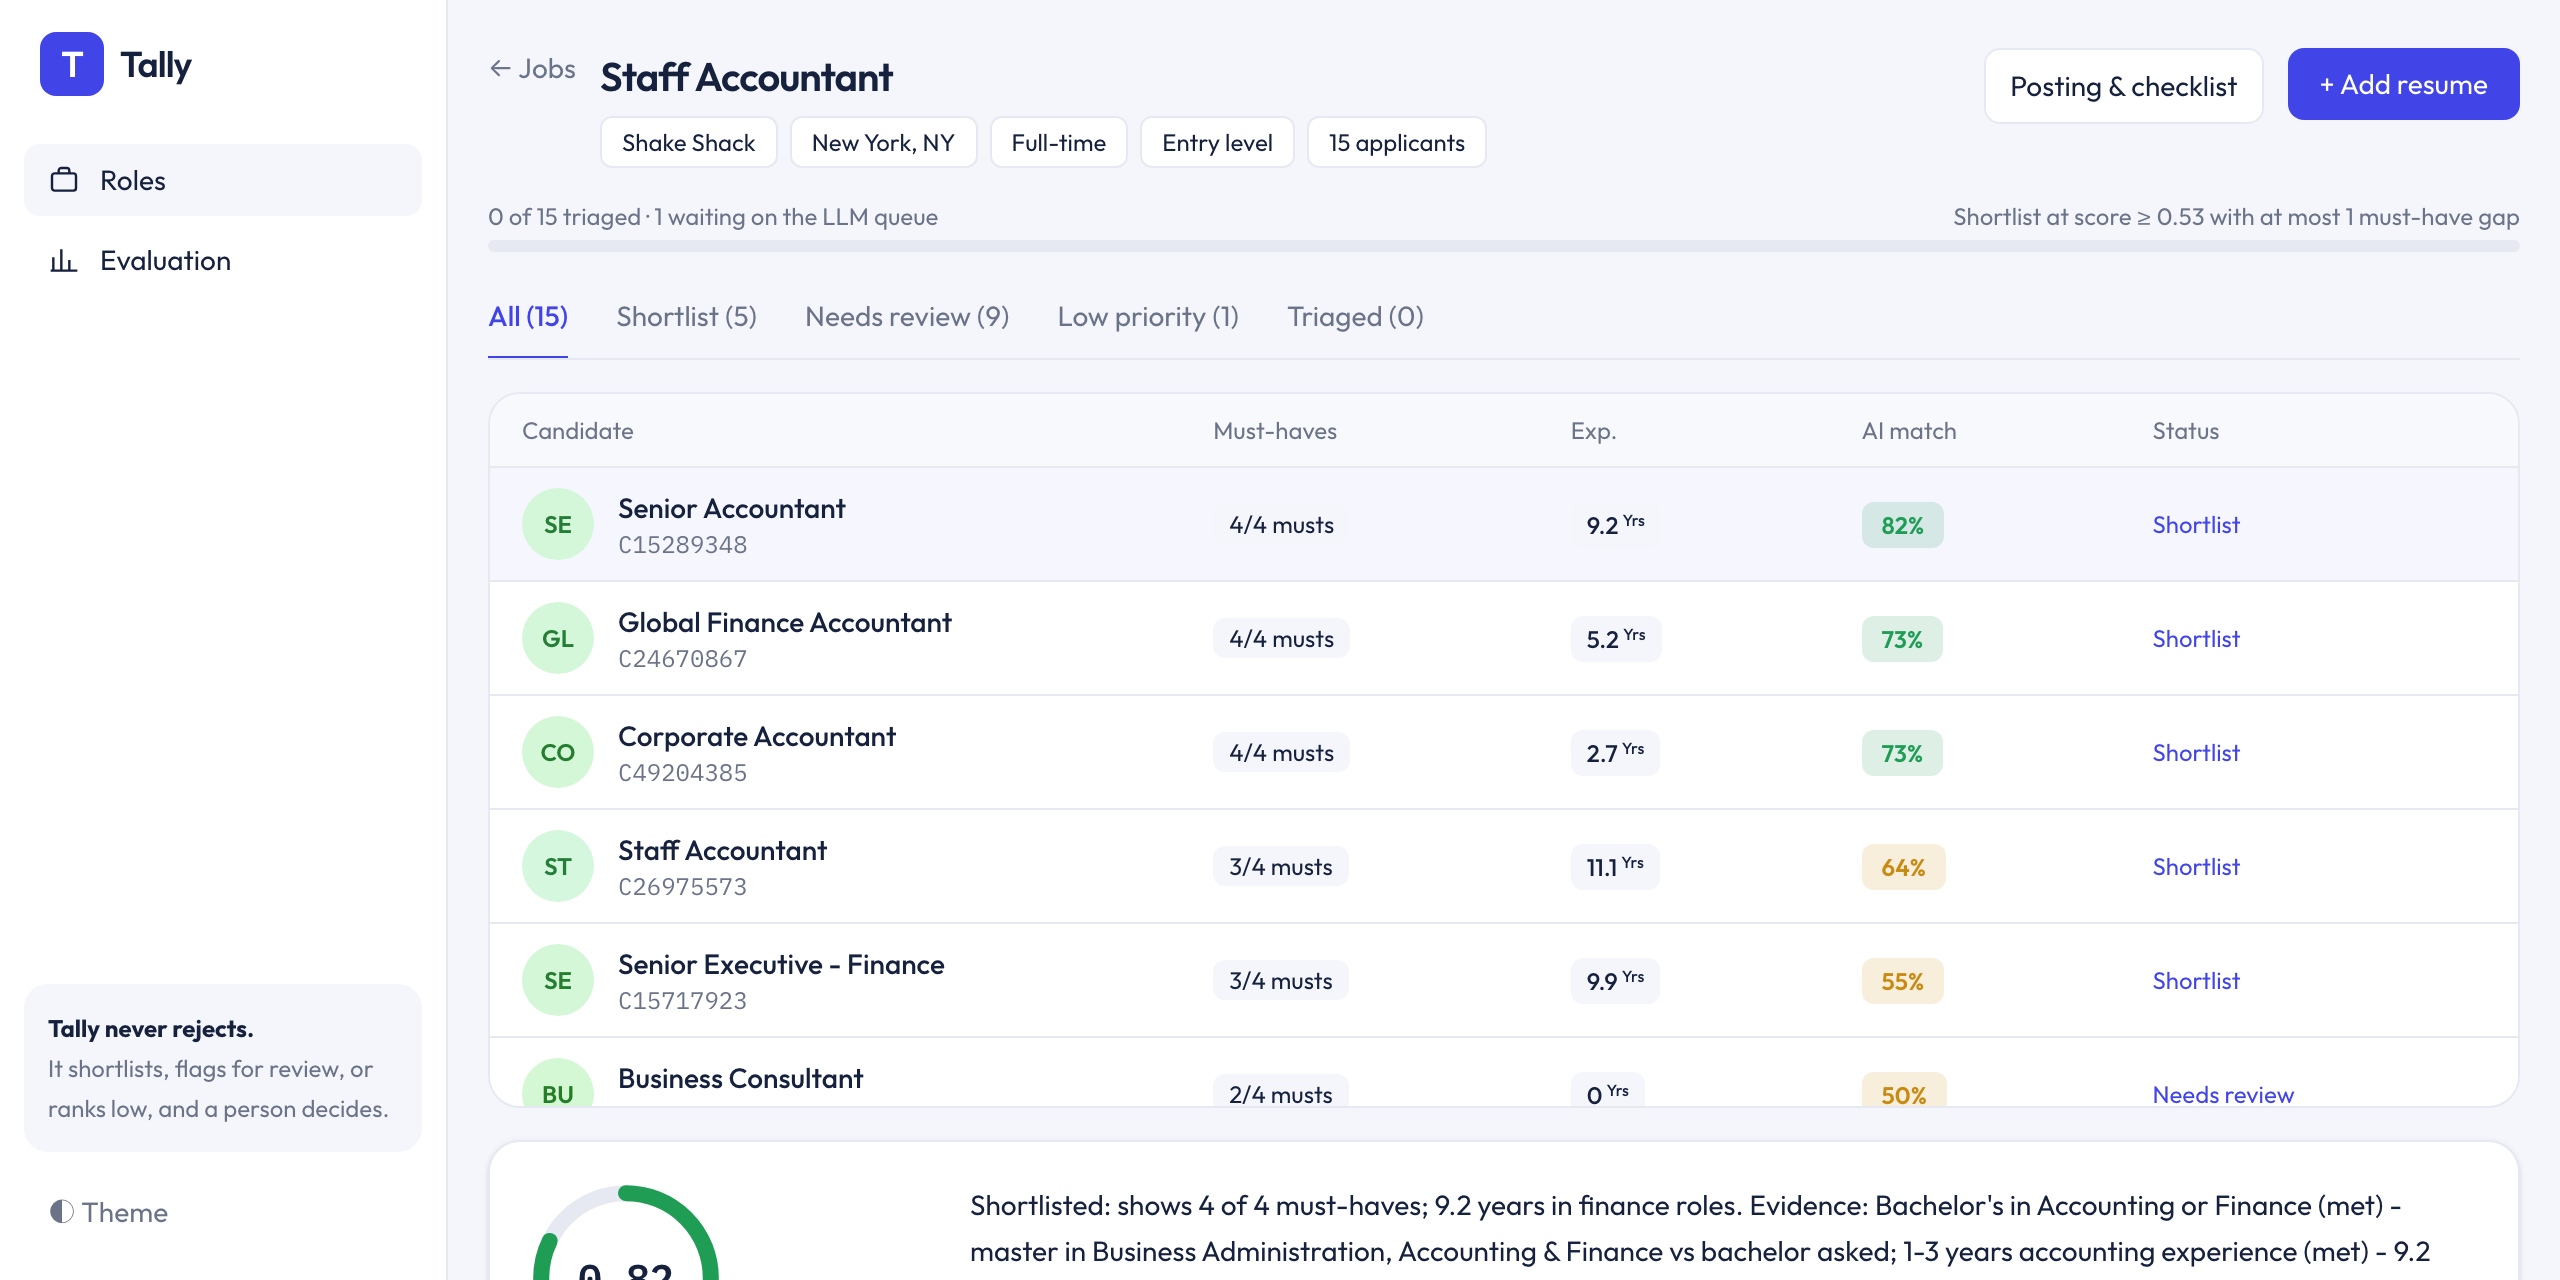
\includegraphics[width=0.49\linewidth]{docs/ui_job.png}
\caption{The Tally interface. Left: roles dashboard with lane counts and shortlist rate. Right: one role's applicants, with must-haves met, relevant years, match score and lane.}
\end{figure}
\end{homeworkProblem}

%----------------------------------------------------------------------------
\begin{homeworkProblem}[3. Golden set]
\begin{itemize}
\item \textbf{Sampling} (\code{tally/golden.py}, independent of the system): per job, 5 BM25-top and 5 random from the ACCOUNTANT/FINANCE pool, 3 from near categories (banking, consulting, sales, business development), and 2 hard cases (the most BM25-similar non-finance resume, and a finance resume whose headline matches the title but ranks outside BM25's top 30). Each resume is used for at most 2 jobs: 129 distinct resumes.
\item \textbf{Labels} (\code{golden/rubric.md}): relevance 0--3 and a decision (advance $\rightarrow$ shortlist, escalate $\rightarrow$ review), with a note per pair, written by a person from text-only packets with no access to scores. Distribution: 0: 60, 1: 48, 2: 42, 3: 30, with \textbf{63 ideal shortlists} (all 30 relevance-3 pairs and 33 of the relevance-2 pairs).
\item \textbf{Second rater.} A Claude Sonnet session labelled the same 180 pairs under the same rubric, also blind (\code{results/label\_agreement.json}). Relevance weighted $\kappa$ \textbf{0.90} (77\% exact, 100\% within $\pm1$). Decision $\kappa$ \textbf{0.90} (95.6\% agreement). The disagreements are systematic, not random: the human scored relevance one point lower on 39 pairs (mean 1.23 vs 1.43), yet shortlisted 8 relevance-2 candidates the model sent to review. Every model shortlist is also a human shortlist. The human is stricter about fit but more willing to let a phone call settle one gap.
\item \textbf{Hard cases} include overqualified directors for associate roles, CPA \emph{candidates} for CPA-required roles, foreign credentials (Philippine CPA, ACCA), finance titles over non-finance duties, and career changers.
\end{itemize}
\end{homeworkProblem}

%----------------------------------------------------------------------------
\begin{homeworkProblem}[4. Results against baselines (test: 9 jobs, 135 pairs)]
\begin{table}[H]
\centering\tablefont\setlength{\tabcolsep}{3.8pt}
\begin{tabular}{lcccccccc}
\toprule
system & NDCG@5 [95\% CI] & P@5 & Spearman & shortlisted & sl.\ precision & recall & sent to a human & cost \\
\midrule
\best{Tally} & \best{0.80} [0.70, 0.89] & \best{0.64} & \best{0.69} & 37 & \best{0.59} & 0.55 & 73\% & 105 \\
TF-IDF cosine & 0.76 [0.67, 0.84] & 0.60 & 0.61 & 82 & 0.39 & 0.80 & 39\% & 90 \\
keyword overlap & 0.70 [0.59, 0.80] & 0.62 & 0.54 & 103 & 0.36 & 0.93 & 24\% & \best{81} \\
\bottomrule
\end{tabular}
\caption*{\footnotesize CIs bootstrap whole jobs. Baseline thresholds were tuned on dev with the same cost rule. ``sl.'' = shortlist.}
\end{table}
\vspace{-6pt}
\begin{itemize}
\item \textbf{Ranking is clearly better.} The checklist separates ``is an accountant'' from ``has what this posting asks for''. Lexical baselines can't: every accounting resume shares the vocabulary.
\item \textbf{Decisions lose on the cost metric} (105 vs 90 and 81). There are 40 good test candidates; Tally shortlists 37 people and gets 22 right (precision 0.59, recall 0.55). At 5:1 cost, every missed good candidate outweighs five wrong shortlists, so the baselines win by shortlisting 61--76\% of all applicants, which a recruiter would not call a shortlist. Tally is the most precise list of the three, but it misses too many good people, and the cost rule I chose up front says that matters more. That is the main open problem (\S8, \S10).
\item \textbf{No good candidate is buried.} None of the 40 went to Low priority; the 18 that were missed are all in Needs review, with reason codes.
\item \textbf{Per job}: NDCG@5 is $\geq 0.85$ on 5 of 9 jobs (J12 accounting manager 1.00, J03 payroll/AP 0.92), but J07 FP\&A manager scores 0.47 (\S8.1) and J10 payroll 0.65.
\end{itemize}
\end{homeworkProblem}

%----------------------------------------------------------------------------
\begin{homeworkProblem}[5. Decision policy and how it was chosen]
The first policy shortlisted only when \textbf{every} must-have was fully met. Its test result was precision 0.70, recall 0.21, 93\% sent to review and cost 133, measured on the AI-drafted labels available at the time; on the human labels it would be 9/10 correct, recall 0.23 and cost 156. Safe but useless, and worse than both baselines. A single \emph{partial} must-have (a ``CPA candidate'', a tool listed but not used) blocked the shortlist, while the rubric lets a recruiter shortlist someone whose one gap ``a phone call settles''.

I then compared gate variants \textbf{on the dev jobs only}, re-tuning the threshold on dev for each. The choice was made on the draft labels; the table re-runs it on the human labels (\code{results/thresholds.json}), and the ranking of the options is the same.

\begin{table}[H]
\centering\tablefont
\begin{tabular}{lcccc}
\toprule
gate (dev, 45 pairs, human labels) & threshold & cost & precision & recall \\
\midrule
all must-haves met (v1) & 0.725 & 90 & 1.00 & 0.22 \\
\best{$\leq$ 1 must-have not fully met (chosen)} & 0.525 & 35 & 1.00 & 0.70 \\
$\leq$ 2 not fully met & 0.40 & 13 & 0.88 & 0.91 \\
score only & 0.45 & 15 & 0.81 & 0.91 \\
\bottomrule
\end{tabular}
\end{table}
\vspace{-4pt}
I chose the one-gap rule over the cheaper options because a shortlist missing two must-haves is not one a recruiter can trust, and it matches the rubric. On the human labels two gaps would cost a third as much on dev. I did \textbf{not} switch after seeing the human test results, because that would be tuning on test; ``precise'' vs ``complete'' is a product decision (\S10). \textbf{Disclosure:} the v1 test numbers had been seen before the policy change, so the test figures are not a fully clean held-out result. v1 and the draft-label results are archived in \code{results/v1\_all\_musts\_gate/} and \code{results/archive\_sonnet\_draft\_labels/}.
\end{homeworkProblem}

%----------------------------------------------------------------------------
\begin{homeworkProblem}[6. Extraction (against the gold files; the gold is still AI-drafted, pending review)]
\begin{table}[H]
\centering\tablefont
\begin{tabular}{lp{4.2in}}
\toprule
field & result \\
\midrule
JD must-haves (12 postings) & precision 0.84, recall 0.63, F1 0.72 \\
all JD requirements & precision 0.82, recall 0.59, F1 0.69 \\
certifications (21 resumes) & F1 0.86 \\
software & precision 0.62, recall 0.99, F1 0.77 (the extractor lists more tools than the gold does) \\
highest education level & 95\% \\
finance-relevant years & MAE 1.55\,y; 76\% within 1 year \\
\bottomrule
\end{tabular}
\end{table}
\vspace{-4pt}
The checklist is the weak link: it finds about two-thirds of what a recruiter would screen on, and its misses become ranking errors downstream (\S8.3). Per-model extraction results are in Table~\ref{tab:models}.
\end{homeworkProblem}

%----------------------------------------------------------------------------
\begin{homeworkProblem}[7. Explanations and the LLM judge]
Explanations are assembled by code from the graded checklist (``Shows 3 of 4 must-haves\ldots\ Evidence: \ldots\ Gaps: \ldots\ Ask about: \ldots''), so they can't invent anything the grader didn't say. \textbf{All 30 sampled explanations' quotes are verified verbatim against the resume} (0 of 180 graded pairs had an unverifiable quote). The \textbf{judge} (\code{tally/prompts.py: judge}) reads the full resume, while the screener only saw retrieved passages, so it can catch evidence the screener missed. Agreement with the \textbf{human reviewer} on 30 test explanations, stratified by lane (\code{results/judge.json}):

\begin{table}[H]
\centering\tablefont
\begin{tabular}{lccccc}
\toprule
dimension & human mean & judge mean & weighted $\kappa$ & within $\pm1$ & Spearman \\
\midrule
grounded & 3.07 & 3.13 & \best{0.52} & 90\% & 0.47 \\
gaps correct & 3.73 & 3.37 & 0.14 & 80\% & 0.09 \\
actionable & 3.57 & 3.07 & 0.29 & 97\% & 0.37 \\
\bottomrule
\end{tabular}
\end{table}
\vspace{-4pt}
\begin{itemize}
\item \textbf{The judge is usable for groundedness only.} It matches the human's mean and ranks explanations moderately well ($\kappa$ 0.52). On gap correctness and actionability it is close to chance, and harsher than the human on both.
\item \textbf{An AI reference would have flattered it.} Against the earlier Sonnet-written reference ratings, the same judge scored $\kappa$ 0.62 / 0.48 / 0.38. The human and that Sonnet reference agree only at $\kappa$ 0.21 / 0.19 / 0.01. Same-family agreement is not human agreement.
\item \textbf{What the human caught.} Explanations are quote-safe, but the \emph{claims} are not always right. The commonest theme (17 of 30 comments) is how years are used: general finance years presented as role-specific tenure (``4+ years of audit''), i.e.\ failure mode 1 from the reader's side. Two code defects also surfaced. (a) The degree check compares level but not field, so a civil-engineering master's ``met'' both ``Bachelor's in accounting'' and ``Master of Tax'' (J05/C28973180, grounded 1). (b) An explanation reported ``9 years in finance roles'' while the same card flagged the role dates as unusable (J07/C14181049). Both are listed for the next iteration (\S10); they were not fixed after the test evaluation.
\end{itemize}
\end{homeworkProblem}

%----------------------------------------------------------------------------
\begin{homeworkProblem}[8. Failure analysis (test set, real examples)]
\begin{enumerate}
\item \textbf{``Years in a similar role'' counted as years in any finance role.} The profile marks each role only as finance / not finance, so years requirements are judged too generously. J07 FP\&A manager (asks 7 years including leadership): four candidates the labeller rated 0--1 were shortlisted, among them accountants, a business consultant and a purchasing manager, all on general finance years (e.g.\ C13130984, an accounting clerk who became an accountant, scored 0.86). That drags J07 to NDCG@5 0.47. \emph{Hypothesis}: extract per-role function tags (FP\&A, payroll, audit, tax\ldots) and match years to the requirement's function.
\item \textbf{The one allowed gap can be the core of the job.} J10 payroll specialist shortlisted two CPAs with no payroll experience (C21794875 rated 1, C16426777 rated 0): the only unmet must-have was ``payroll laws'', but the rest of the checklist (degree, Excel, years) carried the score. \emph{Hypothesis}: the title skill (payroll, tax, audit) should be a hard requirement the one-gap rule can never waive.
\item \textbf{Retrieval misses evidence phrased differently.} J04 (AR accountant, state agency) has the most misses: 6 of its good candidates went to review. C24703009 (relevance 3: Alaska statewide accounting system, multiple funding sources) got ``GAAP not shown'' and ``MS Office not shown'' because no passage contained those words, and was sent to review at 0.45. 18 good test candidates were not shortlisted, and none went to Low priority. \emph{Hypothesis}: always include the skills section as a passage, and accept implied evidence for generic tools.
\item \textbf{Checklist extraction promotes niche or trivial items to must-haves.} J02's ``Timberline (Sage 300)'' was graded as a strict must-have. It is a gap for all four J02 accountants the labeller would advance but Tally sent to review (C27637576, C49204385, C53640713, C78257294, all relevance 2). For C78257294 it is the only gap, and it pulls the score to 0.50, just under the line; the other three also have a second gap (no bachelor's, or ``5+ years in a similar role''). In their notes the labeller accepted QuickBooks, Dynamics or PeopleSoft as ``close enough''. An Office/Excel must-have appears in 6 of the 12 checklists and fails on resumes that never name the tool. Must-have recall against the gold is 0.63. \emph{Hypothesis}: give the checklist step an ``equivalent accepted'' field and drop tool requirements every applicant meets.
\item \textbf{Credentials in progress.} ``CPA candidate'' and ``CPA-eligible'' grade as \emph{partial}. Under the one-gap rule, J12 shortlisted four CPA candidates (C28969385, C23416654, C15289348, C29821051) for a role requiring a professional accreditation; the labeller rated all four 2 but escalated them (``the CPA is not yet held, which the JD requires''). \emph{Hypothesis}: treat credentials as binary (held / not held), with ``in progress'' shown as a note.
\end{enumerate}

\textbf{Manipulation} (synthetic edits of 4 low-fit real resumes, \code{results/adversarial.json}). A visible injection and a zero-width-split injection were flagged 8/8. A paraphrased claim (``the committee already verified this applicant'') was \textbf{not} flagged (0/4) but also moved no scores. Pasting the job's requirements as a skills line raised scores by +0.31 and shortlisted 2 of 4 until a stuffing check was added: it flags any single line that contains $\geq$ 50\% of the requirements, and now flags 4/4 with 0 shortlisted. On the real golden resumes the highest such ratio is 0.20, so it changes no golden decision. A paraphrased stuffing attack would get past it.

\textbf{Fairness} (\code{results/fairness.json}, 6 plausible applicants on 6 test jobs, chosen by BM25 not by score). The swaps were a name line (6 names across gender and ethnicity), a gender cue (Girl Scouts vs Boy Scouts treasurer) and the college on an added degree line (Harvard / Arizona State / Howard / Grand Canyon).
\begin{itemize}
\item \textbf{Gender cue and college: score spread 0.000 and 0 lane flips on both models.}
\item \textbf{Names: a real leak, found by the Gemini run and now fixed.} A name on the first line merged into the first retrieved passage (``Emily Walsh ACCOUNTANT Professional Summary\ldots''), so it \emph{did} reach the grader. Under Sonnet the answers happened not to change. Under Gemini, one applicant (J04/C23734441) scored 0.94 and was shortlisted as Greg Baker, Lakisha Washington, Jamal Robinson or Priya Patel, but 0.72 and sent to review as Emily Walsh or Wei Zhang (max spread 0.22, 1/6 bases flipped). The mechanism was prompt sensitivity, not a judgement about names: with the name in the prompt, Gemini stitched two resume fragments into one ``quote'', verification rejected it, and the candidate went to review. The outcome still depended on the name, so it counts as a fairness failure.
\item \textbf{Fix:} a first line that looks like a person's name is masked to \code{[NAME]} before any LLM call (Title Case job titles are kept; no real resume in the sample is affected, so no headline number moved). \textbf{After the fix: spread 0.000 and 0 flips on both models} (pre-fix results in \code{results/pre\_name\_mask/}).
\item \textbf{Colleges, on the production model:} after the name fix, Gemini 3.5-flash-lite still moved one applicant from review to shortlist when the degree line said Harvard instead of Arizona State, Howard or Grand Canyon (\S11). Institution masking is the open fix.
\item \textbf{Limits:} names elsewhere in a resume (a signature, a reference) are not masked; there are only 6 bases; and the test only proves the pipeline is blind to these edits, not that the labels or the postings are unbiased.
\end{itemize}
\end{homeworkProblem}

%----------------------------------------------------------------------------
\begin{homeworkProblem}[9. What is misleading about my headline number?]
\begin{itemize}
\item \textbf{NDCG@5 0.80 is mostly ``finance beats non-finance''.} Every job's pool contains 3--5 resumes from other fields (near categories, hard look-alikes), so any decent system puts them last. The harder question, which accountant fits \emph{this} accounting job, is where J07 (0.47) and J10 (0.65) show the real weakness.
\item \textbf{The decision policy was revised after seeing test results} (\S5). The rule was chosen on dev, but I only looked for a new rule because v1 looked bad on test.
\item \textbf{Dev is tiny.} 45 pairs and 23 good candidates set the threshold. Dev precision is 1.00, test precision is 0.59, and the bootstrap CI on NDCG@5 spans 0.70--0.89.
\item \textbf{The labels changed the story, so the label source matters.} On the AI-drafted labels Tally narrowly beat both baselines on cost (82 vs 85/88). On the human labels it loses (105 vs 90/81), even though the two label sets agree at $\kappa$ 0.90. A few systematic differences (the human advancing ``one gap a phone call settles'' more often) were enough to flip the decision result. Any small golden set is that sensitive.
\item \textbf{The extraction gold is still AI-made}, so \S6 measures agreement with Sonnet, not with a person. \S7 shows how much that can matter: the judge's $\kappa$ against Sonnet ratings was roughly double its $\kappa$ against the human.
\item \textbf{The numbers are for one model.} Swapping to Gemini changes the lane of 39\% of pairs. 3.1-flash-lite keeps the ranking (NDCG@5 0.80, cost 110); 3.5-flash-lite, the production setting, drops to 0.75 (cost 116) and showed a college-prestige flip (\S11). A ``the agent is good enough'' claim is a claim about a model + prompt pair, not about the design.
\item \textbf{Cost differences are coarse.} One more or one fewer missed good candidate moves the cost by 5, and the 15-point gap to TF-IDF is three candidates.
\item \textbf{The labels reward the checklist's view of the world.} The rubric asks ``does the resume show each must-have'', which is the same question the system answers. A recruiter who weighs trajectory or company quality would label differently.
\end{itemize}
\end{homeworkProblem}

%----------------------------------------------------------------------------
\begin{homeworkProblem}[10. With one more week]
\begin{enumerate}
\item \textbf{Recover recall without giving up precision.} The 18 missed good candidates all sit in Needs review with reason codes. Fixes 3 and 4 below target most of them, and the recruiter could choose the gate (one gap vs two) per job: ``precise list'' or ``complete list''. Fix the two explanation defects the human found (degree field ignored; years stated when dates are unusable), and get a human-checked JD/extraction gold so \S6 stops being measured against a model.
\item \textbf{Make the checklist model-stable.} Most cross-model disagreement starts at checklist extraction (Gemini marks 7 of J02's 8 requirements as must-haves, Sonnet 3 of 5). A recruiter-confirmed checklist (one click per posting) would remove the biggest source of variance and of error at once.
\item Fix failure modes 1, 2 and 5 (function-tagged years, a non-waivable title skill, binary credentials), then evaluate on 4 \emph{new} labelled jobs, because the current test set is no longer clean.
\item Add the skills section to every retrieval and measure the recall change against judge-flagged ``missed evidence''.
\item A larger fairness suite: 30 bases, swaps inside the education field and the profile itself, and a check that extracted degree/years don't change when the name does.
\end{enumerate}
\end{homeworkProblem}

%----------------------------------------------------------------------------
\begin{homeworkProblem}[11. Cross-model check: Claude Sonnet vs two Gemini models]
Same code, prompts, golden set (human labels) and policy, with every LLM step answered by each model in turn. The threshold was re-tuned on the dev jobs per model and landed on 0.525 each time. The production setting is now \code{gemini-3.5-flash-lite}, chosen because \code{3.1-flash-lite} was too often overloaded (503) to rely on. Sources: \code{results/gemini/} (3.5-flash-lite), \code{results/gemini\_3.1\_flash\_lite/}, \code{results/model\_comparison.json}.

\begin{table}[H]
\centering\tablefont
\begin{tabular}{lccc}
\toprule
test (9 jobs, 135 pairs) & Sonnet & Gemini 3.1-flash-lite & Gemini 3.5-flash-lite \\
\midrule
NDCG@5 [95\% CI] & \best{0.80} [0.70, 0.89] & \best{0.80} [0.73, 0.87] & 0.75 [0.63, 0.84] \\
P@5 / Spearman & \best{0.64} / 0.69 & 0.62 / \best{0.71} & 0.58 / 0.62 \\
shortlisted / correct (of 40 good) & 37 / 22 & 42 / 22 & 54 / 23 \\
shortlist precision / recall & \best{0.59} / 0.55 & 0.52 / 0.55 & 0.43 / \best{0.57} \\
sent to a human & 73\% & 69\% & 60\% \\
cost (5 $\times$ missed + 1 $\times$ wrong) & \best{105} & 110 & 116 \\
dev cost (what was tuned) & 35 & 27 & 26 \\
\midrule
\multicolumn{4}{l}{\emph{extraction vs gold}} \\
JD must-haves F1 & 0.72 & 0.71 & 0.72 \\
certifications F1 & 0.86 & 0.86 & \best{0.93} \\
highest education level & \best{95\%} & 81\% & 90\% \\
finance-relevant years MAE (within 1\,y) & \best{1.55\,y (76\%)} & 3.14\,y (52\%) & 2.56\,y (57\%) \\
\bottomrule
\end{tabular}
\caption{Cross-model results (test set) and extraction against the gold.}\label{tab:models}
\end{table}
\vspace{-6pt}
\textbf{Agreement with Sonnet (all 180 pairs).} 3.5-flash-lite: score Spearman 0.84, same lane 61\%, 48 shortlist flips. 3.1-flash-lite: 0.84, 61\%, 45 flips. Both Gemini models mark more requirements as must-haves on some postings (J07 6 vs 2; J02 5--7 vs 3). Dev cost improves with each Gemini model, but test cost gets worse: the threshold tuned on 3 dev jobs does not carry over, and 3.5-flash-lite shortlists 54 people to find 23 good ones.

\textbf{Fairness on 3.5-flash-lite: one prestige flip.} On J09 (senior internal auditor), base C26231609 scored 0.80 and was \textbf{shortlisted with ``Harvard University''} on its degree line, but 0.70 and sent to review with Arizona State, Howard or Grand Canyon (college max spread 0.10, 1/6 bases flipped). The degree line was retrieved as evidence for ``knowledge of accounting principles, COSO, SOX, PCAOB''. With the \emph{same} supporting quote, the model graded it ``met'' next to Harvard and ``partial'' next to the others. Name and gender-cue swaps showed no movement; Sonnet and 3.1-flash-lite showed no movement on any swap. \textbf{Mitigation (not yet applied):} mask institution names before grading, the way names are masked (\S8). That changes the grading prompts, so it means re-running all three models. It is the first item before 3.5-flash-lite goes to production.

\textbf{Judge vs the human reviewer} (weighted $\kappa$ grounded / gaps / actionable): Sonnet 0.52 / 0.14 / 0.29; 3.1-flash-lite 0.31 / 0.11 / 0.22; 3.5-flash-lite $-0.01$ / $-0.09$ / 0.09. 3.5-flash-lite is also extremely lenient (means 4.2--4.7 vs the human's 3.1--3.7). As prompted, only the Sonnet judge is usable, and only for groundedness. \textbf{Manipulation} holds on all three models: injections 8/8 flagged, stuffing 4/4 flagged, 0 shortlisted.

\textbf{Takeaways.} (1) The checklist design beats the lexical baselines on ranking with Sonnet and 3.1-flash-lite, but 3.5-flash-lite (0.75) is within the TF-IDF CI. (2) No model beats the baselines on decision cost under the human labels. (3) Fairness depends on the model, not only on the design: the same pipeline was blind to college names under two models and not under the third. Every model change needs the fairness suite re-run, which this one did.
\end{homeworkProblem}

\end{document}
